{
\section{Projektübersicht}

\begin{frame}
    \tableofcontents[currentsection]
\end{frame}

\begin{frame}{Projektziele und Funktionen}
\begin{columns}

  \column{0.5\textwidth}
  \textbf{Ziele}
  \begin{itemize}
    \item Unterstützung der Cybersicherheits-Ausbildung
    \item Praktische Pentesting-Übungen
    \item Einsatz von portabler Hardware (Raspberry Pi)
    \item Demonstration von Cyberangriffen
  \end{itemize}

  \column{0.5\textwidth}
  \textbf{Funktionen}
  \begin{itemize}
    \item Flexibles, modulares System
    \item Einfache Handhabung
    \item Drahtlose Protokolle (WLAN)
    \item Webanwendungen (OWASP Juice Shop)
  \end{itemize}
  \vspace{.7cm}
\end{columns}
\end{frame}

\begin{frame}{Hardware}
    \begin{figure}[h]
        \centering
        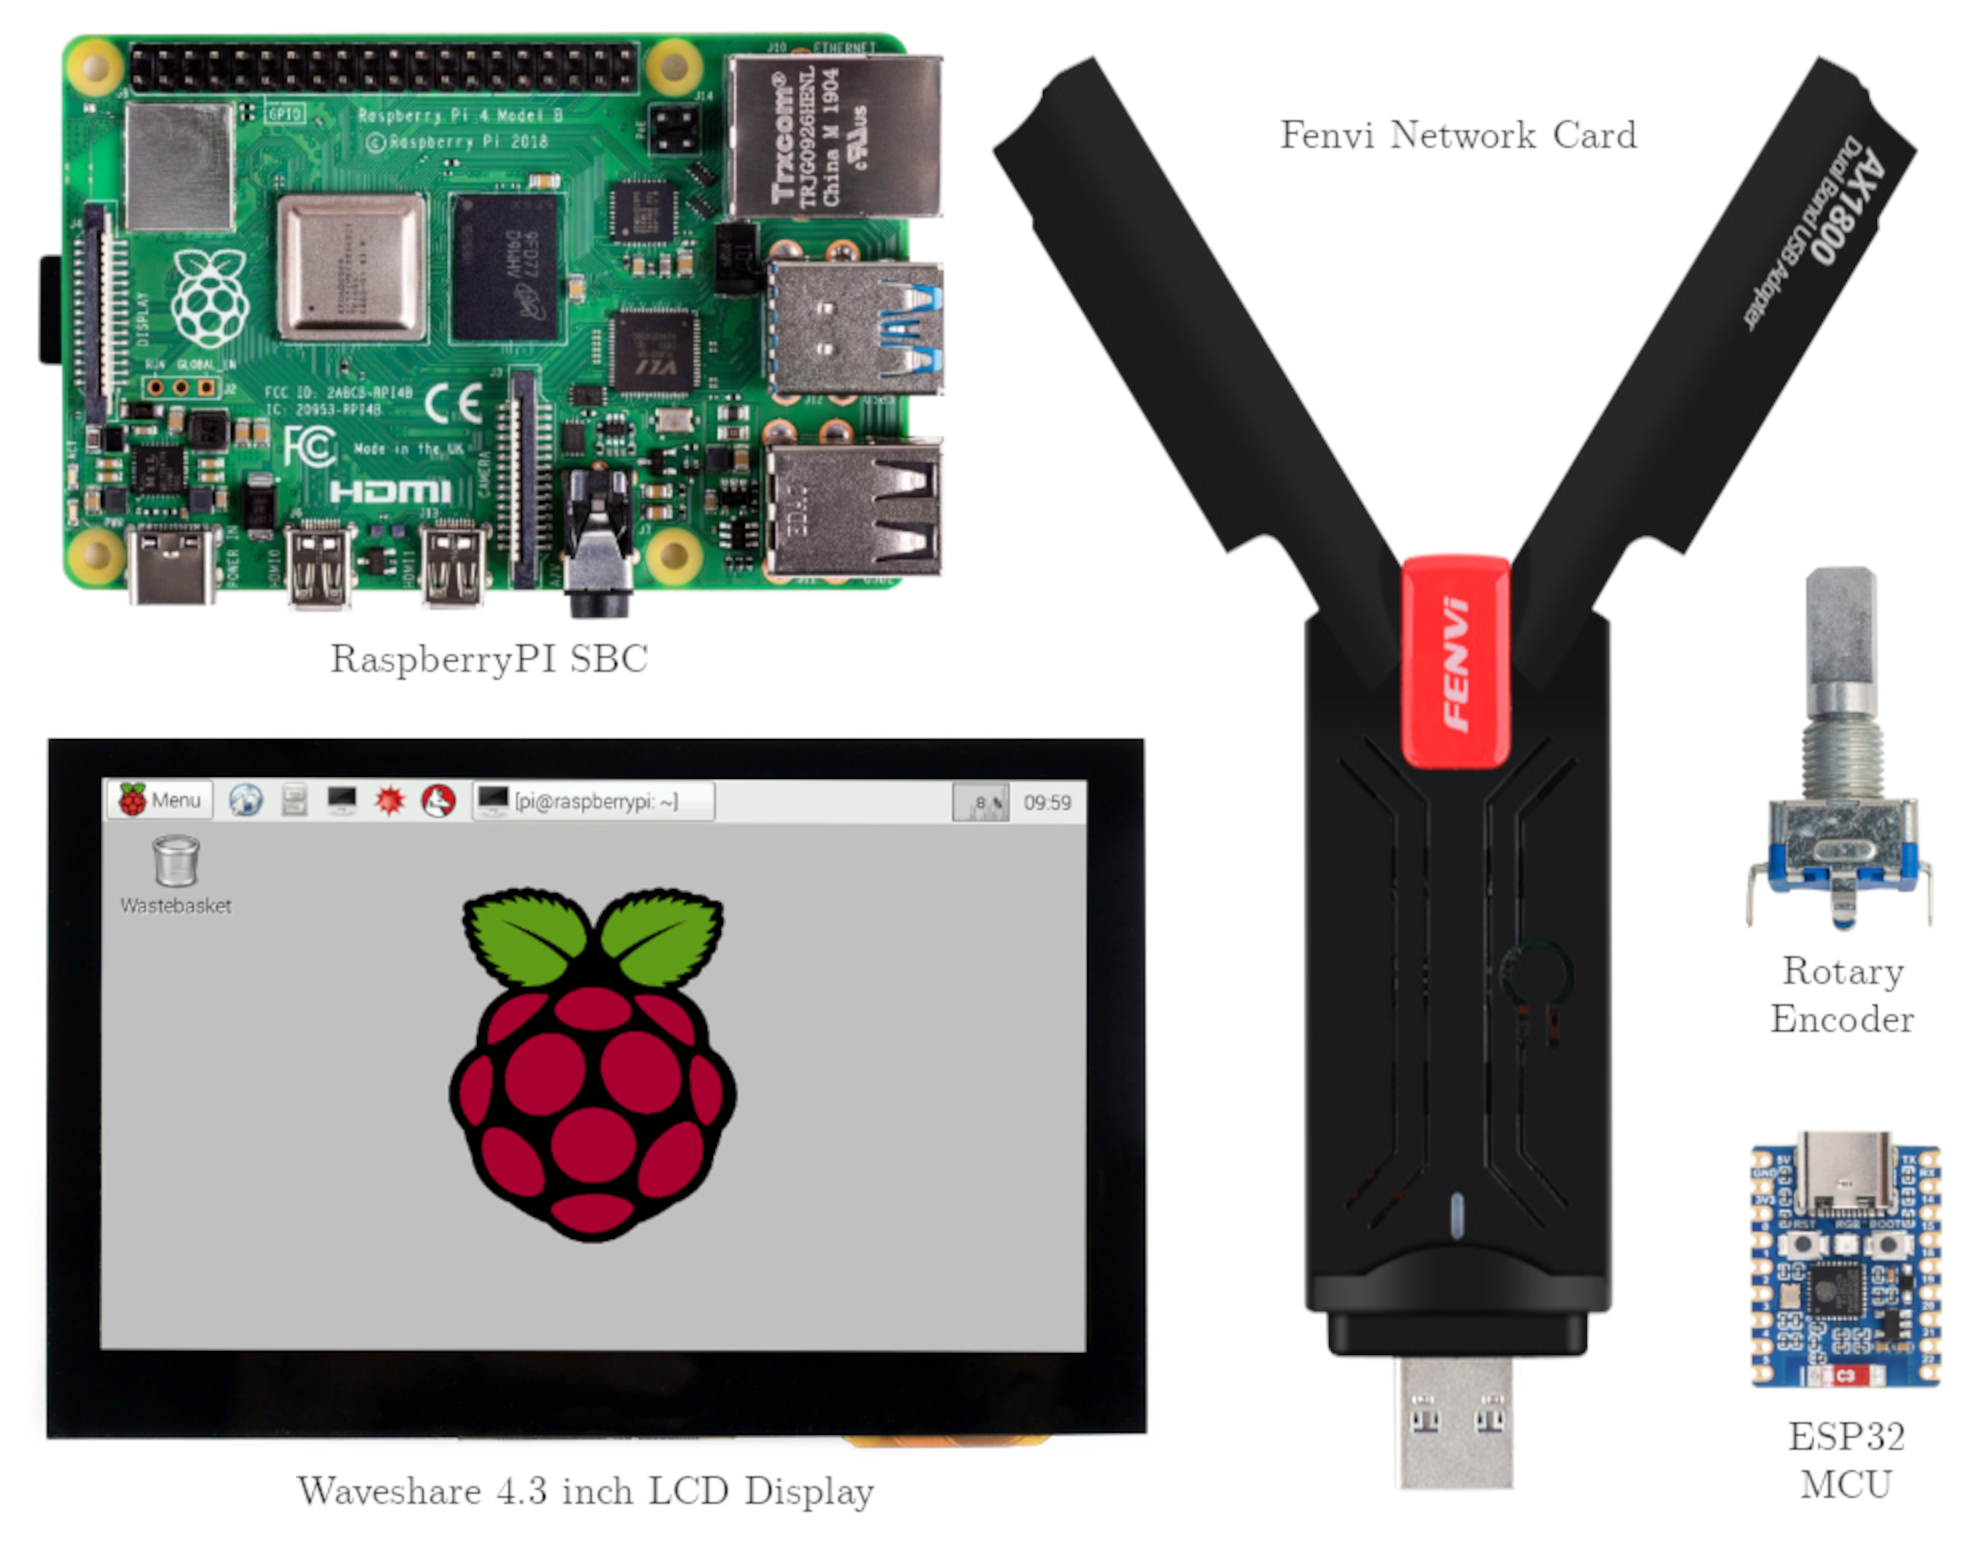
\includegraphics[height=0.8\textheight]{figures/Devices.png}
    \end{figure}
\end{frame}

\begin{frame}{Software}
   \centering
   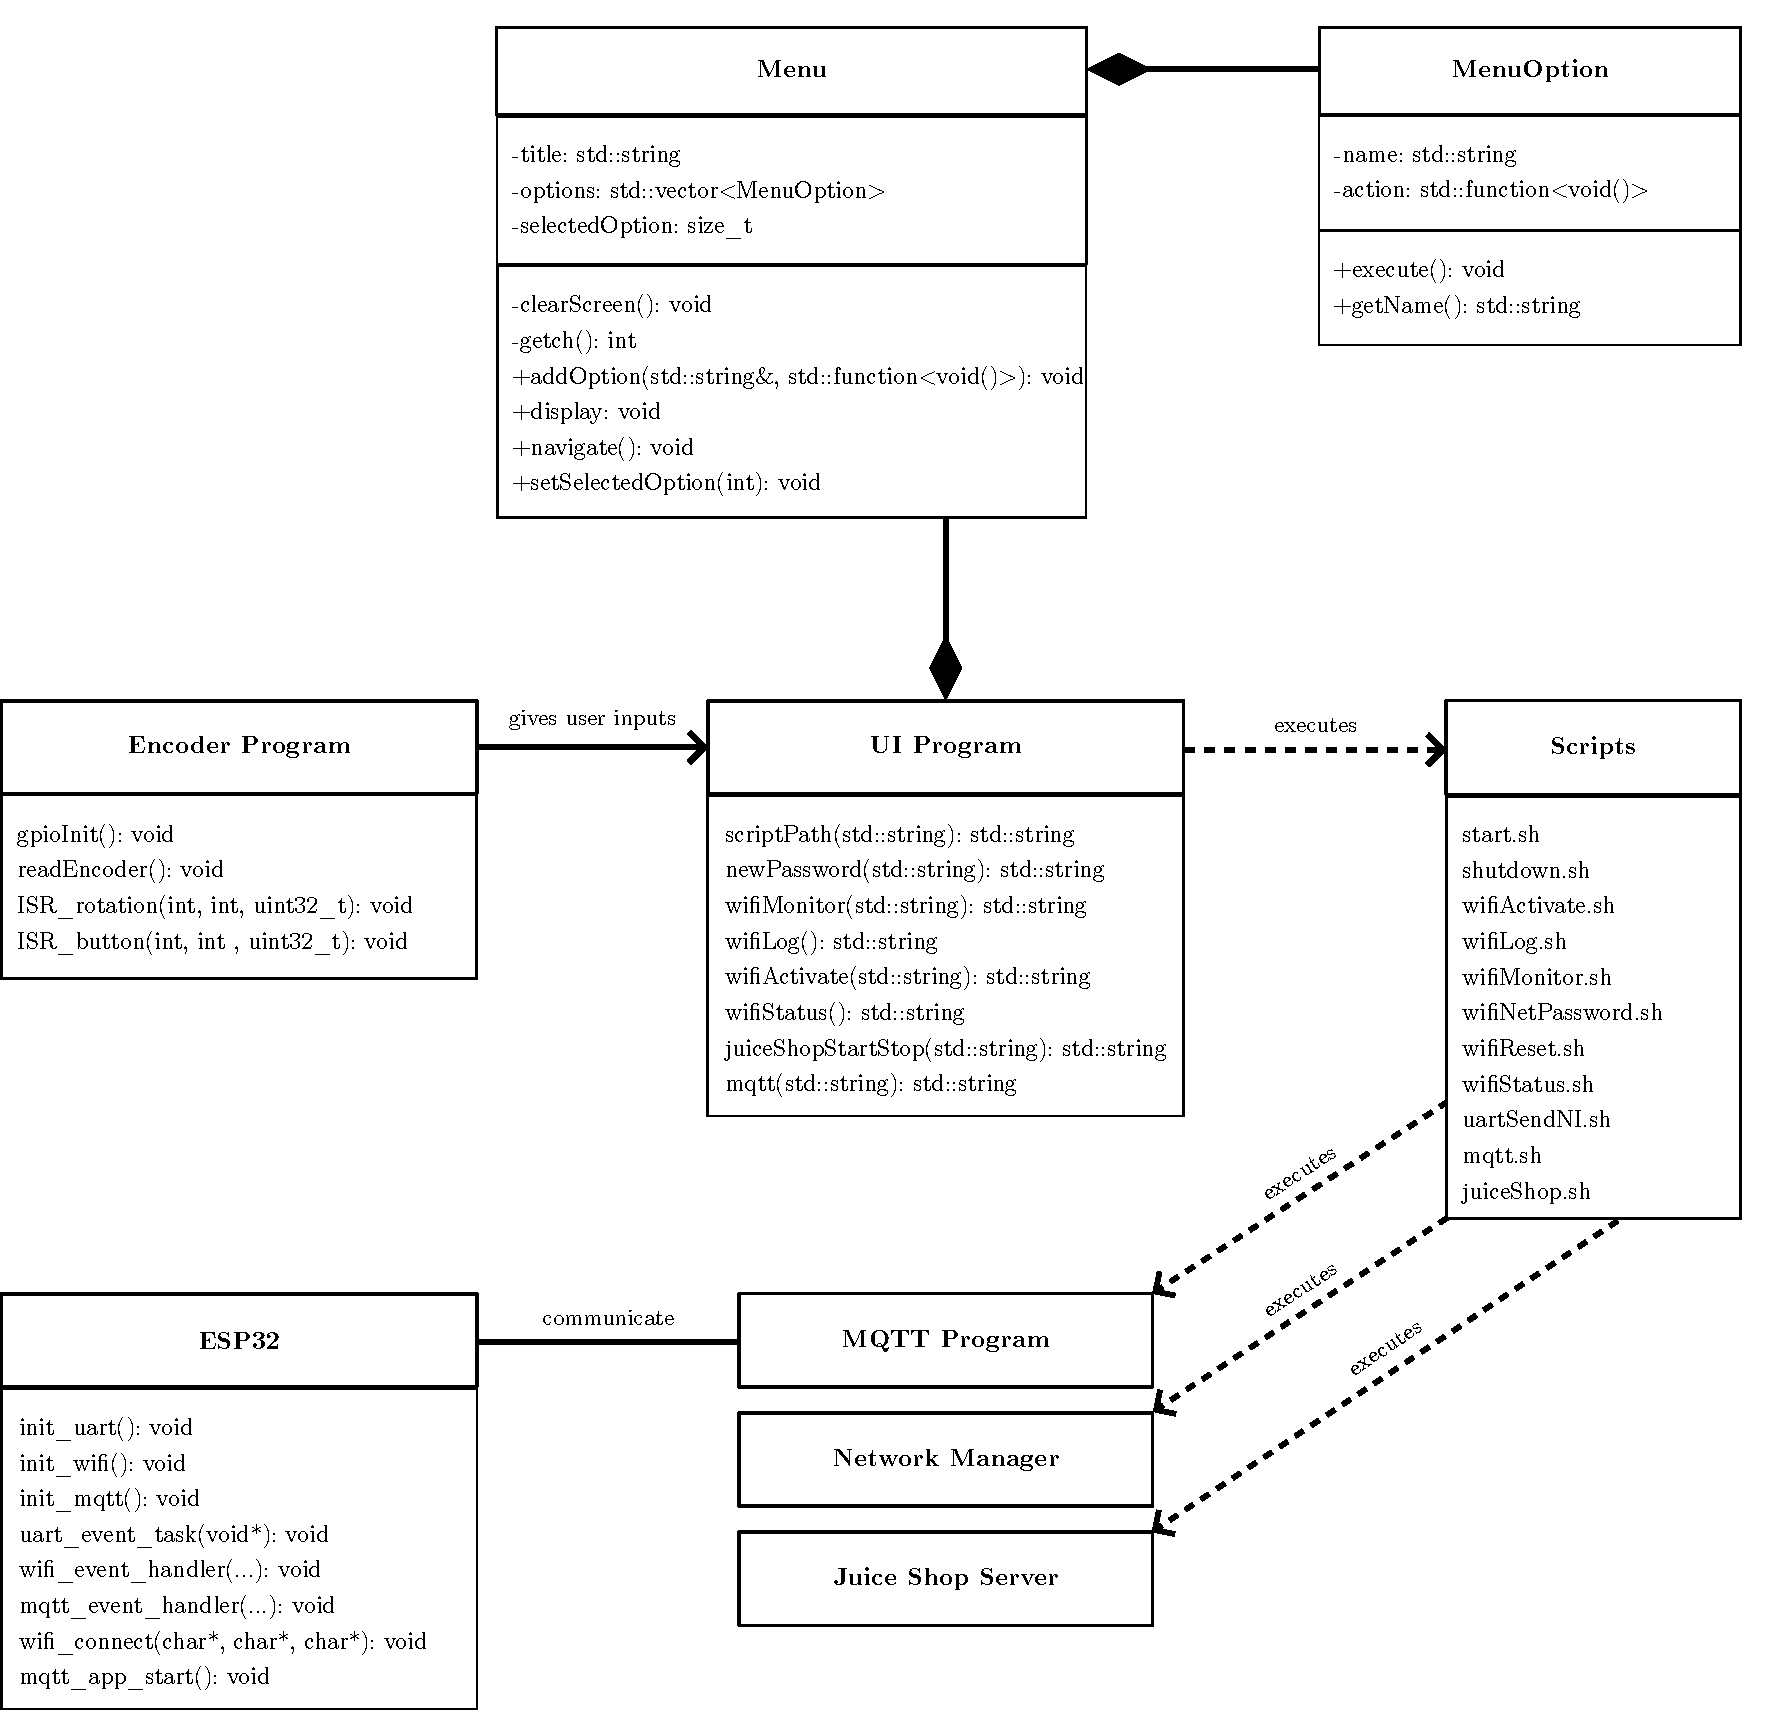
\includegraphics[width=0.9\textwidth]{figures/architecture.pdf}
\end{frame}

\begin{frame}
    \centering
    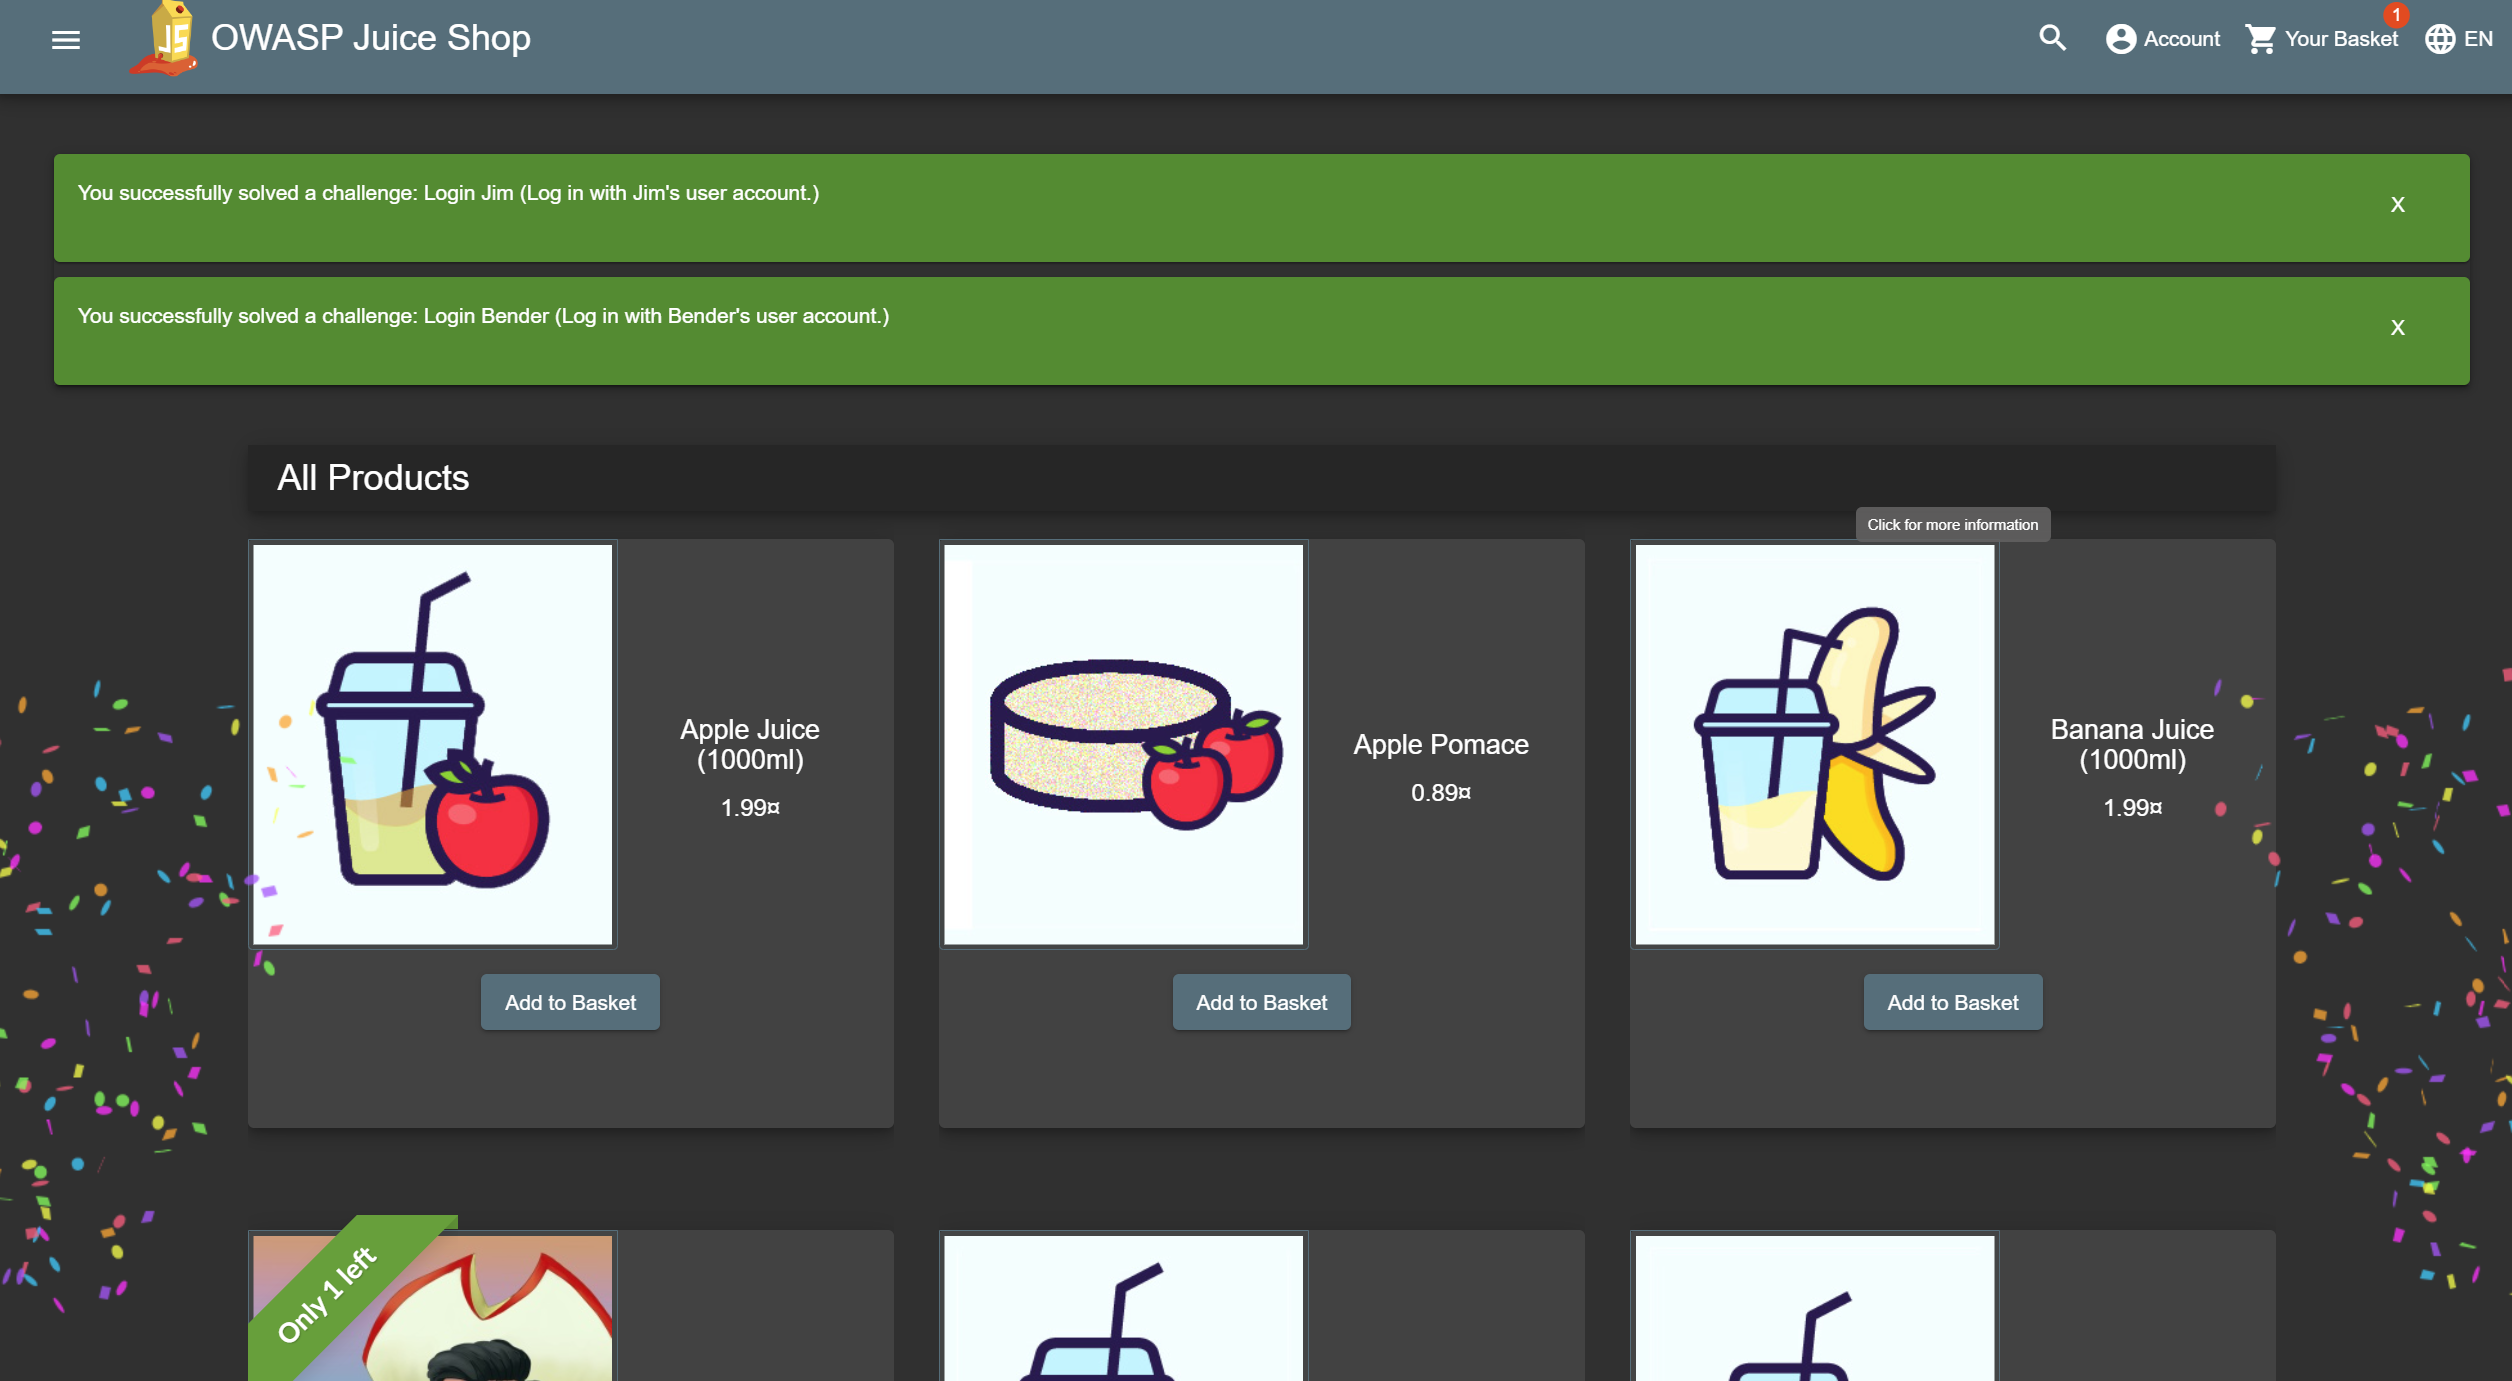
\includegraphics[width=\textwidth]{figures/JuiceShop_2.png}
    \fontsize{4}{4}\selectfont Quelle: https://github.com/OWASP/www-project-juice-shop/blob/master/tab\_overview.md
\end{frame}
}